% =====================================================================
%  SHAP-Guided Corrective RAG for Explainable Clinical Triage
%  IEEE conference format (IEEEtran) -- compile with pdfLaTeX + BibTeX
%  Every experimental value is marked \tbd{} and MUST be replaced with
%  your own measured results before submission. Search for "\tbd".
% =====================================================================
\documentclass[conference]{IEEEtran}
\IEEEoverridecommandlockouts

\usepackage{cite}
\usepackage{amsmath,amssymb,amsfonts}
\usepackage{graphicx}
\usepackage{booktabs}
\usepackage{multirow}
\usepackage{array}
\usepackage{xcolor}
\usepackage{url}
\usepackage{algorithm}
\usepackage{algpseudocode}
\usepackage{tikz}
\usetikzlibrary{arrows.meta,positioning,shapes.geometric,calc,fit}

% ---- placeholder macro: red "TBD" for every value you still need to measure
\newcommand{\tbd}{\textcolor{red}{\textbf{TBD}}}

\begin{document}

\title{Predictive Clinical Triage with SHAP-Guided\\
Corrective Retrieval-Augmented Generation}

\author{
\IEEEauthorblockN{V. Aditya Yaswardhan\IEEEauthorrefmark{1},
Prakrut Dave\IEEEauthorrefmark{1},
Dr. Harriet Linda C\IEEEauthorrefmark{2}}
\IEEEauthorblockA{\IEEEauthorrefmark{1}Computing Technologies, School of Computing,\\
SRM Institute of Science and Technology, Kattankulathur 603203, Tamil Nadu, India}
\IEEEauthorblockA{\IEEEauthorrefmark{2}Assistant Professor, School of Computing,\\
SRM Institute of Science and Technology, Kattankulathur 603203, Tamil Nadu, India}
}

\maketitle

% ---------------------------------------------------------------------
\begin{abstract}
Early recognition of patients who are deteriorating in the intensive care
unit (ICU) depends on two abilities that current AI tools rarely offer
together: reliable reasoning over numeric physiological measurements and
transparent access to the clinical evidence behind a recommendation.
Gradient-boosted classifiers handle tabular vitals well but return an
unexplained probability, while large language models (LLMs) write fluent
explanations yet are unreliable with raw numbers and prone to unsupported
statements. This paper presents a six-stage decision-support pipeline that
links the two. A LightGBM model estimates the probability of sepsis onset
within the next six hours from hourly ICU observations; TreeSHAP isolates
the physiological drivers of each individual prediction; a deterministic
SHAP-to-query bridge turns those drivers into a patient-specific clinical
search query; and a corrective retrieval-augmented generation (CRAG) stage
grades every retrieved passage with a biomedical cross-encoder, keeping,
refining, or replacing evidence through a live PubMed fallback before a
locally constrained LLM writes a source-cited summary. The framework is
evaluated on the PhysioNet/Computing in Cardiology Challenge 2019 cohort
with a cross-hospital split. The selected risk model (XGBoost) reaches an
AUROC of 0.800 (95\% CI 0.789--0.811) on the held-out hospital, SHAP-guided queries improve nDCG@5 by
\tbd{} over generic queries, and corrective routing raises RAGAS
faithfulness from \tbd{} to \tbd{} relative to standard RAG. The system is
intended to support, not replace, clinician judgement.
\end{abstract}

\begin{IEEEkeywords}
Clinical Decision Support, Sepsis Prediction, Explainable AI, SHAP,
Retrieval-Augmented Generation, Corrective RAG, BioBERT, LightGBM, PubMed
\end{IEEEkeywords}

% ---------------------------------------------------------------------
\section{Introduction}

Sepsis, defined as life-threatening organ dysfunction caused by a
dysregulated host response to infection~\cite{singer2016sepsis3}, remains
one of the leading causes of death among critically ill patients. Outcomes
depend heavily on how quickly the condition is recognised: international
guidance stresses early identification followed by prompt fluid
resuscitation, antimicrobial therapy, and haemodynamic
support~\cite{evans2021ssc}. In a busy ICU, however, clinicians must
continuously interpret dozens of vital signs and laboratory values for
every patient, and subtle multi-variable patterns that precede
deterioration are easy to miss.

Machine learning has been applied extensively to this problem. Tree
ensembles and deep networks trained on electronic health records can
anticipate adverse events hours ahead of clinical
recognition~\cite{nemati2018aise,rajkomar2018ehr,reyna2020physionet}.
Yet a bare probability gives a clinician little to act on. Without knowing
\emph{why} a model raised an alarm, staff cannot judge whether the alarm is
plausible, and surveys of clinicians identify this opacity as a key barrier
to adoption~\cite{tonekaboni2019clinicians}.

Large language models appear to fill this gap, since they can express
clinical reasoning in natural language and have achieved strong results on
medical question answering~\cite{singhal2023medpalm}. They are, however,
poorly suited to direct risk estimation from tabular measurements, and they
can generate confident statements that are not grounded in any
source~\cite{ji2023hallucination}. Retrieval-augmented generation
(RAG)~\cite{lewis2020rag} mitigates the second problem by conditioning the
LLM on retrieved documents, but standard RAG passes the top-ranked passages
to the generator regardless of their quality. When the query is vague or
the knowledge base lacks coverage, irrelevant evidence flows straight into
the answer~\cite{yan2024crag}.

We argue that these weaknesses are complementary and can be resolved by
assigning each sub-task to the component best suited to it. Our pipeline
uses a gradient-boosted model for numeric risk estimation, SHAP for
per-patient attribution, a rule-based bridge for converting attributions
into a retrieval query, a biomedical cross-encoder for judging evidence
quality, and an LLM only for the final, evidence-bound synthesis. The
overall architecture is shown in Fig.~\ref{fig:arch}.

The main contributions of this paper are:
\begin{itemize}
\item A \textbf{SHAP-to-RAG bridge} that converts the top positive SHAP
attributions of an individual prediction into a deterministic,
terminology-controlled clinical query, so that retrieval is driven by the
same evidence that drove the risk score.
\item A \textbf{clinically adapted corrective retrieval stage} in which a
biomedical cross-encoder grades retrieved passages and routes each case to
one of three actions, including a MeSH-based query rewrite and live PubMed
fallback when local evidence is insufficient.
\item A \textbf{privacy-aware generation design} in which the LLM never
receives raw patient records, only derived feature descriptions and graded
passages, with a post-hoc check that each cited sentence is supported.
\item An \textbf{ablation-based evaluation protocol} that separately
measures predictive performance, retrieval relevance, and answer
faithfulness, isolating the contribution of each component.
\end{itemize}

The rest of the paper is organised as follows. Section~II reviews related
work. Section~III describes the dataset. Section~IV details the
methodology. Section~V presents the experimental setup and results,
Section~VI discusses findings and limitations, and Section~VII concludes.

% ---------------------------------------------------------------------
\begin{figure*}[!t]
\centering
\resizebox{\textwidth}{!}{%
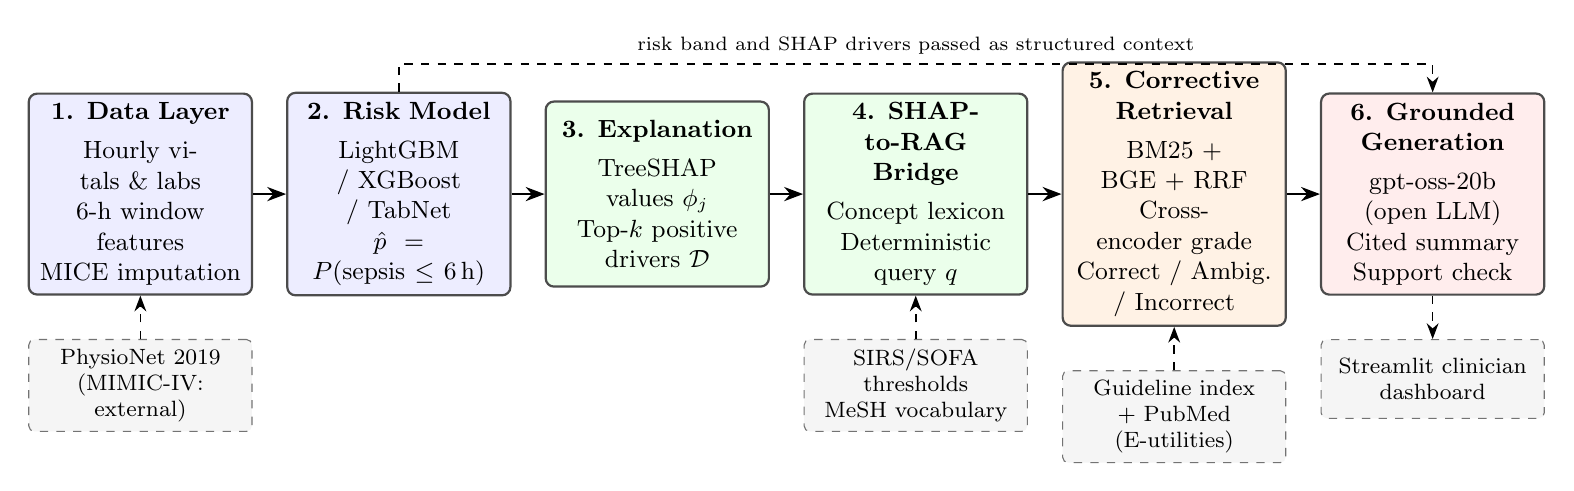
\begin{tikzpicture}[
  node distance=0.42cm,
  stage/.style={rectangle, rounded corners=3pt, draw=black!70, thick,
                fill=#1, minimum height=2.35cm, align=center,
                font=\small, text width=2.6cm},
  src/.style={rectangle, rounded corners=2pt, draw=black!55, dashed,
              fill=gray!8, minimum height=1.0cm, align=center,
              font=\footnotesize, text width=2.6cm},
  arr/.style={-{Stealth[length=2.4mm]}, thick},
  darr/.style={-{Stealth[length=2.0mm]}, semithick, dashed}
]
\node[stage=blue!7] (s1) {\textbf{1. Data Layer}\\[3pt]
  Hourly vitals \& labs\\ 6-h window features\\ MICE imputation};
\node[stage=blue!7, right=of s1] (s2) {\textbf{2. Risk Model}\\[3pt]
  LightGBM / XGBoost\\ / TabNet\\ $\hat{p}=P(\text{sepsis}\le 6\,\text{h})$};
\node[stage=green!8, right=of s2] (s3) {\textbf{3. Explanation}\\[3pt]
  TreeSHAP values $\phi_j$\\ Top-$k$ positive\\ drivers $\mathcal{D}$};
\node[stage=green!8, right=of s3] (s4) {\textbf{4. SHAP-to-RAG}\\\textbf{Bridge}\\[3pt]
  Concept lexicon\\ Deterministic query $q$};
\node[stage=orange!10, right=of s4] (s5) {\textbf{5. Corrective}\\\textbf{Retrieval}\\[3pt]
  BM25 + BGE + RRF\\ Cross-encoder grade\\ Correct / Ambig. / Incorrect};
\node[stage=red!7, right=of s5] (s6) {\textbf{6. Grounded}\\\textbf{Generation}\\[3pt]
  gpt-oss-20b (open LLM)\\ Cited summary\\ Support check};

\foreach \a/\b in {s1/s2, s2/s3, s3/s4, s4/s5, s5/s6}
  \draw[arr] (\a) -- (\b);

\node[src, below=0.55cm of s1] (d1) {PhysioNet 2019\\ (MIMIC-IV: external)};
\node[src, below=0.55cm of s4] (d4) {SIRS/SOFA thresholds\\ MeSH vocabulary};
\node[src, below=0.55cm of s5] (d5) {Guideline index\\ + PubMed (E-utilities)};
\node[src, below=0.55cm of s6] (d6) {Streamlit clinician\\ dashboard};

\draw[darr] (d1) -- (s1);
\draw[darr] (d4) -- (s4);
\draw[darr] (d5) -- (s5);
\draw[darr] (s6) -- (d6);
\draw[darr] (s2.north) -- ++(0,0.35) -| node[pos=0.25, above, font=\scriptsize]
  {risk band and SHAP drivers passed as structured context} (s6.north);
\end{tikzpicture}}
\caption{Overall architecture of the proposed pipeline. Numeric prediction
and attribution (Stages 1--3) are handled by tabular models; the bridge
(Stage 4) converts attributions into a controlled query; corrective
retrieval (Stage 5) grades and repairs evidence; the LLM (Stage 6) only
synthesises graded evidence and never sees raw patient records.}
\label{fig:arch}
\end{figure*}

% ---------------------------------------------------------------------
\section{Literature Survey}

\subsection{Machine Learning for Sepsis and Deterioration}
Early-warning research has moved from rule-based scores towards learned
models. Nemati et al.~\cite{nemati2018aise} built an interpretable model
that predicted sepsis four to twelve hours in advance from routinely
collected ICU data. Rajkomar et al.~\cite{rajkomar2018ehr} showed that deep
models over full EHR timelines predict mortality and readmission at scale,
and Komorowski et al.~\cite{komorowski2018aiclinician} used reinforcement
learning to study treatment policies for septic patients. The
PhysioNet/Computing in Cardiology Challenge 2019~\cite{reyna2020physionet}
provided a shared benchmark for hourly sepsis prediction, in which
gradient-boosted trees were among the strongest approaches. More broadly,
tree ensembles such as XGBoost~\cite{chen2016xgboost} and
LightGBM~\cite{ke2017lightgbm} often match or outperform deep architectures
on tabular data~\cite{shwartz2022tabular}, while TabNet~\cite{arik2021tabnet}
offers an attention-based deep alternative.

\subsection{Explainability in Clinical Prediction}
SHapley Additive exPlanations (SHAP)~\cite{lundberg2017shap} assign each
input feature a contribution to an individual prediction based on
cooperative game theory. TreeSHAP~\cite{lundberg2020treeshap} computes
these values exactly and efficiently for tree ensembles, and has been used
to explain intra-operative hypoxaemia alerts to
anaesthesiologists~\cite{lundberg2018hypoxaemia}. In existing work,
however, SHAP output is the end of the pipeline: it is displayed to the
user but is not used to drive any further reasoning.

\subsection{Retrieval-Augmented Generation in Medicine}
RAG~\cite{lewis2020rag} combines a retriever with a generator so that
answers are conditioned on external documents; a broad survey of variants
is given by Gao et al.~\cite{gao2023ragsurvey}. In medicine,
Almanac~\cite{zakka2024almanac} used retrieval over curated clinical sources
to improve factuality, and the MIRAGE benchmark~\cite{xiong2024medrag}
systematically compared retrievers, corpora, and LLMs for medical question
answering. Domain-specific encoders such as
BioBERT~\cite{lee2020biobert} and the PubMed-trained MedCPT
retriever~\cite{jin2023medcpt} improve biomedical text matching. In all of
these systems the query is written by a human user.

\subsection{Self-Correcting Retrieval}
Self-RAG~\cite{asai2024selfrag} trains an LLM to emit reflection tokens that
decide when to retrieve and whether a generated segment is supported.
Corrective RAG (CRAG)~\cite{yan2024crag} instead attaches a lightweight
retrieval evaluator that labels retrieved documents as correct, incorrect,
or ambiguous and triggers knowledge refinement or web search accordingly.
CRAG was evaluated on open-domain benchmarks with general web search. Our
work adapts the corrective idea to a clinical setting: the evaluator is a
biomedical cross-encoder, the external source is PubMed with controlled
MeSH vocabulary, and the query itself is produced automatically from a
patient-level explanation.

\subsection{Research Gap}
Table~\ref{tab:compare} summarises the capabilities of representative
approaches. To our knowledge, prior systems either predict risk, explain
predictions, or retrieve evidence, but do not use per-patient attributions
to control what is retrieved and then verify that evidence before
generation. This paper targets that integration.

\begin{table}[!t]
\caption{Capability Comparison with Representative Approaches}
\label{tab:compare}
\centering
\footnotesize
\setlength{\tabcolsep}{3pt}
\begin{tabular}{@{}lccccc@{}}
\toprule
Approach & Risk & Expl. & Auto query & Evid. grading & Citations \\
\midrule
Sepsis ML~\cite{nemati2018aise} & \checkmark & partial & -- & -- & -- \\
TreeSHAP~\cite{lundberg2020treeshap} & \checkmark & \checkmark & -- & -- & -- \\
Medical RAG~\cite{zakka2024almanac,xiong2024medrag} & -- & -- & -- & -- & \checkmark \\
CRAG~\cite{yan2024crag} & -- & -- & -- & \checkmark & partial \\
Self-RAG~\cite{asai2024selfrag} & -- & -- & -- & \checkmark & \checkmark \\
\textbf{This work} & \checkmark & \checkmark & \checkmark & \checkmark & \checkmark \\
\bottomrule
\end{tabular}
\end{table}

% ---------------------------------------------------------------------
\section{Dataset}

\subsection{Primary Cohort}
Experiments use the publicly available PhysioNet/Computing in Cardiology
Challenge 2019 dataset~\cite{reyna2020physionet,goldberger2000physionet}.
It contains de-identified hourly records for 40{,}336 adult ICU patients
from two separate hospital systems (Hospital A: 20{,}336 patients;
Hospital B: 20{,}000 patients). Each hourly row holds up to 40 variables:
8 vital signs (e.g., heart rate, systolic and mean arterial pressure,
temperature, respiratory rate, SpO$_2$), 26 laboratory values (e.g.,
lactate, white-cell count, platelets, creatinine, bilirubin), and 6
demographic or administrative fields (age, sex, ICU length of stay,
hospital admission time). Sepsis onset is defined by the Sepsis-3
criteria~\cite{singer2016sepsis3}, and the challenge label is set to
positive from six hours before onset onwards, which frames the task as
early warning. Roughly 7\% of patients develop sepsis during their stay,
and the share of positive hourly rows is much smaller, so the data are
strongly imbalanced. Table~\ref{tab:data} summarises the cohort.

\begin{table}[!t]
\caption{Dataset Summary}
\label{tab:data}
\centering
\footnotesize
\begin{tabular}{@{}lcc@{}}
\toprule
Property & Hospital A (train/val) & Hospital B (test) \\
\midrule
Patients & 20{,}336 & 20{,}000 \\
Hourly records & 790{,}215 & 761{,}995 \\
Septic patients (\%) & 1{,}790 (8.80) & 1{,}142 (5.71) \\
Positive hourly rows (\%) & 2.17 & 1.41 \\
Variables per hour & 40 & 40 \\
\bottomrule
\end{tabular}
\end{table}

\subsection{External Validation Cohort}
MIMIC-IV~\cite{johnson2023mimiciv} is used only as an optional external
validation set for the risk model. Because its data use agreement prohibits
sharing records with third-party online services, all MIMIC-IV experiments
run entirely offline with a locally hosted model, and no MIMIC-derived text
is sent to any external API.

\subsection{Evidence Corpus}
The local knowledge base contains openly accessible clinical guidance on
sepsis and critical care, including the Surviving Sepsis Campaign
guidelines~\cite{evans2021ssc} and open-access review articles. Documents
are split into passages of about 256 tokens with a 32-token overlap, and
each passage keeps metadata on its source, section heading, and
publication year so that it can be cited. The local guidance is
supplemented with PubMed abstracts of reviews and guidelines from the last
ten years, retrieved through E-utilities for 17 sepsis-related topics and
8 unrelated critical-care topics that act as realistic distractors. The final
index holds 1{,}315 documents and 2{,}319 passages (51 from guideline notes,
2{,}268 from PubMed). Because the target population is adults, passages whose
titles refer to neonatal or paediatric populations are excluded at
retrieval time.

\subsection{Preprocessing}
Preprocessing follows a strict leakage-free order. (1) Patients are split
by hospital: Hospital A is used for training and validation with an 80/20
patient-grouped split stratified by sepsis status, and Hospital B is held out entirely as an
external test set. (2) Within each patient, measurements are
forward-filled for at most a variable-specific carry window (e.g., 4\,h for
vitals, 24\,h for laboratory values). (3) Remaining gaps are imputed with
Multiple Imputation by Chained Equations (MICE)~\cite{vanbuuren2011mice},
fitted on training folds only. (4) Binary missingness indicators are kept
as features, since the decision to order a test is itself
informative. (5) Class imbalance is handled inside training folds only,
comparing SMOTE~\cite{chawla2002smote} with class-weighted loss; the
validation and test sets are never resampled.

% ---------------------------------------------------------------------
\section{Methodology}

\subsection{Problem Formulation}
Let $\mathbf{x}_{t} \in \mathbb{R}^{m}$ be the feature vector of a patient
at ICU hour $t$, built from the observations in the window $[t-w+1, t]$.
The risk model estimates
\begin{equation}
\hat{p}_t = f(\mathbf{x}_t) \approx P\left(y_t = 1 \mid \mathbf{x}_t\right),
\end{equation}
where $y_t=1$ if sepsis onset occurs within the next six hours. For each
alert the pipeline returns $\hat{p}_t$, a driver set $\mathcal{D}_t$, a
graded evidence set $\mathcal{E}_t$, and a cited summary.

\subsection{Stage 1: Feature Engineering}
For each variable and a trailing window of $w=6$ hours we compute the last
observed value, mean, minimum, maximum, linear slope, and the number of
measurements taken. Static features (age, sex) and ICU length of stay are
appended. This yields $m=210$ features per hourly row. All statistics use
only past and present observations, so no future information leaks into a
prediction.

\subsection{Stage 2: Risk Prediction}
Three candidate models are trained: LightGBM~\cite{ke2017lightgbm}, a
histogram-based gradient-boosting framework with leaf-wise tree growth;
XGBoost~\cite{chen2016xgboost}, a regularised boosting system with
level-wise growth; and TabNet~\cite{arik2021tabnet}, a deep tabular model
that applies sequential attention to select features at each decision step.
The boosting models use a learning rate of 0.05 with up to 2{,}000 trees
and early stopping (patience 100) on the validation area under the
precision--recall curve (AUPRC), which is more informative than accuracy
under heavy imbalance. Each boosting model is trained twice, once with
class-weighted loss and once on SMOTE-resampled training rows (all
positives plus 150{,}000 sampled negatives, minority ratio 0.3). TabNet is
trained on a 250{,}000-row subsample with balanced batch sampling. The
predicted probabilities of the chosen model are calibrated with isotonic
regression. Because missing a septic patient is costlier than a false
alarm, the alert threshold $\theta$ is chosen on validation data as the
highest value that achieves a sensitivity of at least 0.80. The final model
is selected by validation AUPRC, not decided in advance.

\subsection{Stage 3: Patient-Level Explanation}
For the selected tree model, TreeSHAP~\cite{lundberg2020treeshap} computes
the Shapley value of each feature $j$:
\begin{equation}
\phi_j = \sum_{S \subseteq F \setminus \{j\}}
\frac{|S|!\,(|F|-|S|-1)!}{|F|!}
\left[ f_{S\cup\{j\}}(\mathbf{x}) - f_S(\mathbf{x}) \right],
\label{eq:shap}
\end{equation}
where $F$ is the full feature set and $f_S$ is the model's expected output
when only features in $S$ are known. The values satisfy local accuracy,
\begin{equation}
f(\mathbf{x}) = \phi_0 + \sum_{j=1}^{m} \phi_j ,
\end{equation}
with $\phi_0$ the mean model output (in log-odds space). Since engineered
features derive from a small number of raw variables, attributions are
first aggregated per raw variable $v$, $\Phi_v = \sum_{j \in v} \phi_j$.
The driver set keeps the variables that push the prediction towards
sepsis most strongly:
\begin{equation}
\mathcal{D} = \operatorname{top\text{-}k}_{v}
\left\{ \Phi_v \;\middle|\; \Phi_v > \delta \right\},
\label{eq:drivers}
\end{equation}
with $k=3$ and a small margin $\delta$ that excludes negligible
contributions.

\subsection{Stage 4: SHAP-to-RAG Bridge}
A driver only becomes a retrieval term if the patient's actual value is
clinically abnormal; a high SHAP value for a normal temperature, for
instance, should not produce a query about fever. The bridge therefore
applies a concept lexicon (Table~\ref{tab:lexicon}) whose thresholds are
adapted from SIRS and SOFA conventions~\cite{singer2016sepsis3}. Each
driver $v \in \mathcal{D}$ whose latest value $x_v$ satisfies its trigger
is mapped to a plain-language concept $c_v$ and a MeSH
heading~\cite{lipscomb2000mesh} $h_v$. The local query is filled from a
fixed template:

\vspace{2pt}
\noindent\fbox{\parbox{0.95\columnwidth}{\footnotesize\ttfamily
Evidence-based assessment and management of \{$c_1$\}, \{$c_2$\} and
\{$c_3$\} in an adult ICU patient at \{risk band\} risk of sepsis.}}
\vspace{2pt}

\noindent and the PubMed query is built from the MeSH headings, e.g.
\texttt{("$h_1$"[MeSH] AND "$h_2$"[MeSH]) AND ("Sepsis"[MeSH] OR "Shock,
Septic"[MeSH])}, restricted to guidelines and reviews from the last ten
years. Because the bridge is deterministic, the same patient state always
produces the same query, which makes retrieval auditable and avoids
relying on an LLM to invent search terms. If no driver passes its trigger,
the query falls back to the generic risk band alone.

\begin{table}[!t]
\caption{Concept Lexicon Used by the SHAP-to-RAG Bridge}
\label{tab:lexicon}
\centering
\footnotesize
\setlength{\tabcolsep}{3pt}
\begin{tabular}{@{}llll@{}}
\toprule
Variable & Trigger & Concept & MeSH heading \\
\midrule
MAP & $<65$ mmHg & hypotension & Hypotension \\
SBP & $<90$ mmHg & hypotension & Hypotension \\
Lactate & $>2$ mmol/L & raised lactate & Acidosis, Lactic \\
Heart rate & $>90$ /min & tachycardia & Tachycardia \\
Resp. rate & $>20$ /min & tachypnoea & Tachypnea \\
Temperature & $>38$ / $<36$ $^\circ$C & fever / hypothermia & Fever / Hypothermia \\
SpO$_2$ & $<92$\% & hypoxaemia & Hypoxia \\
WBC & $>12$ / $<4$ $\times10^3$/$\mu$L & leukocytosis / -penia & Leukocytosis / Leukopenia \\
Platelets & $<150$ $\times10^3$/$\mu$L & thrombocytopenia & Thrombocytopenia \\
Creatinine & $>1.2$ mg/dL & renal dysfunction & Acute Kidney Injury \\
Bilirubin & $>1.2$ mg/dL & hepatic dysfunction & Hyperbilirubinemia \\
\bottomrule
\end{tabular}
\end{table}

\subsection{Stage 5: Corrective Retrieval}

\subsubsection{Hybrid retrieval}
Two retrievers run in parallel. The lexical retriever uses
BM25~\cite{robertson2009bm25}:
\begin{equation}
\mathrm{BM25}(q,d) = \sum_{t \in q} \mathrm{IDF}(t)\,
\frac{tf_{t,d}\,(k_1+1)}{tf_{t,d} + k_1\left(1-b+b\,\frac{|d|}{\overline{|d|}}\right)},
\end{equation}
with $k_1=1.5$ and $b=0.75$. The dense retriever embeds queries and
passages with BGE-base-en-v1.5~\cite{xiao2023bge} and ranks by cosine
similarity in a vector index (ChromaDB). The two ranked lists are merged by
reciprocal rank fusion~\cite{cormack2009rrf}:
\begin{equation}
\mathrm{RRF}(d) = \sum_{r \in \{\text{bm25},\,\text{dense}\}}
\frac{1}{\kappa + \mathrm{rank}_r(d)}, \qquad \kappa = 60,
\end{equation}
and the top $K=10$ passages are passed to the grader. The lexical retriever
catches exact clinical terms and drug names, while the dense retriever
catches paraphrases such as ``low blood pressure'' for ``hypotension''.

\subsubsection{Relevance grading}
Unlike the bi-encoder used for retrieval, a cross-encoder reads the query
and a passage together and outputs a single relevance
score~\cite{nogueira2019bert}. We fine-tune BioBERT~\cite{lee2020biobert}
as a cross-encoder $g(\cdot,\cdot)$ with weak supervision from the PubMed
corpus: each article title is paired with its own abstract (positive), the
highest-ranked BM25 abstract of a different article (hard negative), and a
random abstract (easy negative). The MedCPT
cross-encoder~\cite{jin2023medcpt}, trained on PubMed search logs, and a
general MS MARCO cross-encoder serve as alternative graders. Grader scores
are mapped to $[0,1]$ with temperature scaling,
\begin{equation}
s_i = \sigma\!\left(\frac{g(q, p_i) - b}{T}\right), \qquad S = \max_{i} s_i ,
\end{equation}
where $\sigma$ is the logistic function. Temperature scaling is needed
because cross-encoder logits are unbounded (MedCPT logits span roughly
$-16$ to $+12$), so a plain sigmoid saturates and the routing thresholds
lose meaning; we use $(b,T)=(-2,4)$ for MedCPT, $(0,1.5)$ for MS MARCO, and
$(0,1)$ for the BCE-trained BioBERT grader.

\subsubsection{Routing}
The case is routed by its best evidence score:
\begin{equation}
\text{route}(S) =
\begin{cases}
\textsc{Correct}, & S \ge \tau_h,\\
\textsc{Ambiguous}, & \tau_l < S < \tau_h,\\
\textsc{Incorrect}, & S \le \tau_l,
\end{cases}
\label{eq:route}
\end{equation}
with initial values $\tau_h = 0.75$ and $\tau_l = 0.35$, later calibrated
on a development set as described in Section~V. The three actions are
shown in Fig.~\ref{fig:crag}:
\begin{itemize}
\item \textsc{Correct}: passages with $s_i \ge \tau_l$ are split into
sentence-level strips, each strip $u$ is re-scored, and only strips with
$\sigma(g(q,u)) \ge \tau_s$ are kept, removing off-topic sentences inside
otherwise relevant passages.
\item \textsc{Ambiguous}: local strips are filtered as above and combined
with graded PubMed abstracts retrieved with the MeSH query, so that weak
local evidence is supplemented rather than discarded.
\item \textsc{Incorrect}: local passages are dropped, the query is
rewritten with MeSH headings and synonyms, and evidence comes only from
graded PubMed results fetched through the NCBI E-utilities
API~\cite{sayers2010eutils}.
\end{itemize}
If no passage from any source exceeds $\tau_l$, the system reports that
insufficient evidence was found instead of generating unsupported advice.

\begin{figure}[!t]
\centering
\resizebox{\columnwidth}{!}{%
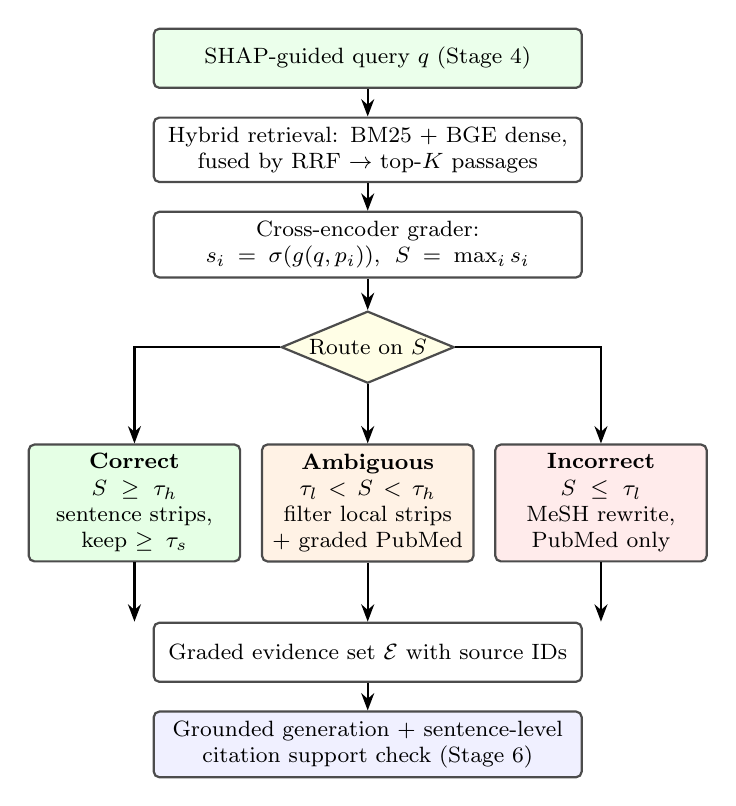
\begin{tikzpicture}[
  box/.style={rectangle, rounded corners=2pt, draw=black!70, thick,
              align=center, font=\footnotesize, text width=#1,
              minimum height=0.75cm},
  box/.default=5.2cm,
  dec/.style={diamond, aspect=2.4, draw=black!70, thick, align=center,
              font=\footnotesize, inner sep=1pt, fill=yellow!10},
  arr/.style={-{Stealth[length=2.2mm]}, thick}
]
\node[box, fill=green!8] (q) {SHAP-guided query $q$ (Stage 4)};
\node[box, below=0.35cm of q] (r) {Hybrid retrieval: BM25 + BGE dense,\\ fused by RRF $\rightarrow$ top-$K$ passages};
\node[box, below=0.35cm of r] (g) {Cross-encoder grader:\\ $s_i=\sigma(g(q,p_i))$,\; $S=\max_i s_i$};
\node[dec, below=0.4cm of g] (d) {Route on $S$};
\node[box=2.45cm, below=0.75cm of d, fill=orange!10] (amb) {\textbf{Ambiguous}\\ $\tau_l<S<\tau_h$\\ filter local strips\\ + graded PubMed};
\node[box=2.45cm, left=0.25cm of amb, fill=green!10] (cor) {\textbf{Correct}\\ $S\ge\tau_h$\\ sentence strips,\\ keep $\ge\tau_s$};
\node[box=2.45cm, right=0.25cm of amb, fill=red!8] (inc) {\textbf{Incorrect}\\ $S\le\tau_l$\\ MeSH rewrite,\\ PubMed only};
\node[box, below=0.75cm of amb] (e) {Graded evidence set $\mathcal{E}$ with source IDs};
\node[box, below=0.35cm of e, fill=blue!6] (gen) {Grounded generation + sentence-level\\ citation support check (Stage 6)};

\draw[arr] (q) -- (r);
\draw[arr] (r) -- (g);
\draw[arr] (g) -- (d);
\draw[arr] (d.west) -| (cor.north);
\draw[arr] (d.south) -- (amb.north);
\draw[arr] (d.east) -| (inc.north);
\draw[arr] (cor.south) -- (cor.south |- e.north);
\draw[arr] (amb.south) -- (e.north);
\draw[arr] (inc.south) -- (inc.south |- e.north);
\draw[arr] (e) -- (gen);
\end{tikzpicture}}
\caption{Corrective retrieval workflow. The best grader score $S$ decides
whether local evidence is kept, supplemented with PubMed, or replaced by
MeSH-rewritten PubMed retrieval.}
\label{fig:crag}
\end{figure}

\subsection{Stage 6: Grounded Generation}
\label{sec:gen}
The generator is gpt-oss-20b~\cite{openai2025gptoss}, an open-weight
(Apache-2.0) mixture-of-experts language model that can be self-hosted,
run with low reasoning effort and with its reasoning trace hidden. Its
prompt contains (i) the risk band and calibrated probability,
(ii) the driver set $\mathcal{D}$ written as concepts with binned values
(e.g., ``lactate 4--5 mmol/L''), and (iii) the graded evidence $\mathcal{E}$
with passage identifiers. No identifiers, timestamps, or raw time series are
included. The model is instructed to write four short sections (risk
summary, contributing observations, relevant evidence, considerations for
clinician review), to attach a passage identifier to every factual
sentence, and to state explicitly when evidence is missing. Generation uses
temperature 0 for reproducibility.

After generation, each sentence $a$ with cited passage $p$ is re-scored by
the grader; sentences with $\sigma(g(a,p)) < \tau_c$ are flagged as
unsupported and removed from the displayed summary. The proportion of
retained, correctly cited sentences is reported as citation precision.
Orchestration of Stages 2--6 is implemented as a state graph in LangGraph,
where the routing rule in~(\ref{eq:route}) selects the next node.
Algorithm~\ref{alg:pipeline} summarises the procedure.

\begin{algorithm}[!t]
\caption{SHAP-Guided Corrective RAG for One Alert}
\label{alg:pipeline}
\footnotesize
\begin{algorithmic}[1]
\Require window features $\mathbf{x}_t$, model $f$, threshold $\theta$, lexicon $L$
\State $\hat{p} \gets f(\mathbf{x}_t)$
\If{$\hat{p} < \theta$} \State \Return low-risk status \EndIf
\State $\boldsymbol{\phi} \gets \textsc{TreeSHAP}(f, \mathbf{x}_t)$; aggregate to $\Phi_v$
\State $\mathcal{D} \gets$ top-$k$ variables with $\Phi_v > \delta$ \Comment{Eq.~(\ref{eq:drivers})}
\State $C \gets \{(c_v, h_v) \in L : v \in \mathcal{D},\ x_v \text{ meets trigger}\}$
\State $q \gets \textsc{Template}(C, \text{band}(\hat{p}))$; $q_{\text{mesh}} \gets \textsc{MeSHQuery}(C)$
\State $P \gets \textsc{RRF}(\textsc{BM25}(q), \textsc{Dense}(q))[1..K]$
\State $s_i \gets \sigma(g(q,p_i))$ for $p_i \in P$; $S \gets \max_i s_i$
\If{$S \ge \tau_h$} \State $\mathcal{E} \gets \textsc{StripFilter}(P, q, \tau_s)$
\ElsIf{$S > \tau_l$} \State $\mathcal{E} \gets \textsc{StripFilter}(P, q, \tau_s) \cup \textsc{Grade}(\textsc{PubMed}(q_{\text{mesh}}))$
\Else \State $\mathcal{E} \gets \textsc{Grade}(\textsc{PubMed}(\textsc{Rewrite}(q_{\text{mesh}})))$
\EndIf
\If{$\mathcal{E} = \emptyset$} \State \Return ``insufficient evidence'' \EndIf
\State $A \gets \textsc{LLM}(\hat{p}, C, \mathcal{E})$
\State \Return $\hat{p}$, $\mathcal{D}$, $\mathcal{E}$, $\textsc{SupportCheck}(A, \mathcal{E}, \tau_c)$
\end{algorithmic}
\end{algorithm}

\subsection{Illustrative Walk-Through}
Consider a synthetic patient (not drawn from any dataset) with heart rate
125/min, systolic pressure 84\,mmHg, mean arterial pressure 60\,mmHg,
temperature 39.0\,$^\circ$C, respiratory rate 28/min, and lactate
4.3\,mmol/L. Suppose the model's probability exceeds $\theta$ and the three
largest positive aggregated SHAP values belong to MAP, lactate, and heart
rate. All three meet their triggers, so the bridge produces the query
\emph{``Evidence-based assessment and management of hypotension, raised
lactate and tachycardia in an adult ICU patient at high risk of
sepsis''} together with the MeSH query on \emph{Hypotension},
\emph{Acidosis, Lactic}, and \emph{Tachycardia}. Temperature, although
abnormal, does not enter the query because its SHAP contribution was
smaller; it is still shown on the dashboard. This example illustrates the
mechanism only and reports no measured output.

% ---------------------------------------------------------------------
\section{Experimental Setup and Results}

% >>> All numbers in this section are placeholders. Replace every \tbd
% >>> with your measured values and rewrite the interpretation sentences
% >>> so that they describe what you actually observed.

\subsection{Implementation}
All components are implemented in Python~3.11 using scikit-learn,
LightGBM, XGBoost, PyTorch-TabNet, SHAP, rank-bm25, ChromaDB,
sentence-transformers, LangGraph, and Streamlit. The generator is served
through the Groq API for PhysioNet experiments; because it is open-weight,
it can be hosted locally for MIMIC-IV experiments. Faithfulness is judged
by the same model with a separate claim-verification prompt. Random seeds are fixed at 42. Table~\ref{tab:config}
lists the main settings.

\begin{table}[!t]
\caption{Main Configuration}
\label{tab:config}
\centering
\footnotesize
\begin{tabular}{@{}ll@{}}
\toprule
Component & Setting \\
\midrule
Feature window & $w=6$ h; last, mean, min, max, slope, count \\
Imbalance & SMOTE vs.\ class weights (train folds only) \\
Model selection & 80/20 grouped split of Hospital A, AUPRC \\
Alert threshold & sensitivity $\ge 0.80$ on validation \\
SHAP drivers & $k=3$, aggregated per raw variable \\
Chunking & 256 tokens, 32 overlap \\
Retrieval & BM25 ($k_1$=1.5, $b$=0.75) + BGE-base, RRF $\kappa$=60, $K$=10 \\
Grader & BioBERT cross-encoder (alt.: MedCPT) \\
Routing thresholds & $\tau_h$=0.75, $\tau_l$=0.35 (initial; calibrated) \\
Generator & gpt-oss-20b (Groq), temperature 0, low reasoning \\
\bottomrule
\end{tabular}
\end{table}

\subsection{Evaluation Protocol}
\subsubsection{Prediction}
Models are compared on the Hospital B test set using AUROC, AUPRC,
sensitivity and specificity at threshold $\theta$, F1-score, and the Brier
score for calibration. 95\% confidence intervals are obtained from 1{,}000
patient-level bootstrap resamples, and AUROC differences are tested with
DeLong's method.

\subsubsection{Retrieval}
An evaluation set of $N=\tbd$ alerts is sampled from Hospital B, stratified
by driver combination. For each alert, the top-10 passages from every
system are pooled and labelled for relevance on a 0--2 scale by two
annotators, with disagreements adjudicated \tbd. We report nDCG@5 and
Precision@5. The same labels are used to calibrate $\tau_h$ and $\tau_l$ on
a development split of the alerts.

\subsubsection{Generation}
Summaries are scored with RAGAS~\cite{es2024ragas} (faithfulness, answer
relevancy, context precision) and with citation precision as defined in
Section~\ref{sec:gen}. A subset of \tbd{} summaries is additionally reviewed for
clinical correctness by \tbd.

\subsubsection{Ablations}
Four factors are varied one at a time: (A1) query source---generic
``sepsis management'' query, all abnormal variables without SHAP ranking,
an LLM-written query, and the proposed SHAP-guided query; (A2)
retriever---BM25, dense, hybrid; (A3) correction---standard RAG, grader
filtering only, full CRAG with PubMed fallback; and (A4) grader---a general
MS MARCO cross-encoder, MedCPT, and BioBERT.

\subsection{Predictive Performance}
Table~\ref{tab:pred} reports test-set results. The best model by validation
AUPRC was XGBoost trained on SMOTE-resampled rows, which reached an AUROC of
0.800 (95\% CI 0.789--0.811) and an AUPRC of 0.077 (95\% CI 0.069--0.086) on
the external hospital, against a positive-row prevalence of 1.41\%. The four
boosting configurations performed within 0.007 AUROC of each other, so the
choice between class weighting and SMOTE had little effect, whereas TabNet
trailed by about 0.04 AUROC, consistent with reports that tree ensembles
remain strong on tabular data~\cite{shwartz2022tabular}. The threshold
chosen for 0.80 sensitivity on Hospital A yielded a sensitivity of 0.64 at a
specificity of 0.82 on Hospital B, showing that alert thresholds drift
across sites and should be recalibrated locally before deployment.

\begin{table}[!t]
\caption{Predictive Performance on the Held-Out Hospital (B)}
\label{tab:pred}
\centering
\footnotesize
\setlength{\tabcolsep}{3.5pt}
\begin{tabular}{@{}lcccccc@{}}
\toprule
Model & AUROC & AUPRC & Sens. & Spec. & F1 & Brier \\
\midrule
LightGBM + SMOTE & 0.796 & 0.075 & 0.652 & 0.798 & 0.083 & 0.0136 \\
LightGBM + weights & 0.793 & 0.075 & 0.607 & 0.826 & 0.088 & 0.0135 \\
\textbf{XGBoost + SMOTE} & \textbf{0.800} & \textbf{0.077} & 0.644 & 0.819 & \textbf{0.090} & 0.0135 \\
XGBoost + weights & 0.792 & 0.071 & 0.645 & 0.804 & 0.084 & 0.0135 \\
TabNet & 0.757 & 0.063 & 0.731 & 0.659 & 0.057 & 0.0136 \\
\bottomrule
\end{tabular}
\end{table}

\subsection{Explanation Analysis}
TreeSHAP was computed for a random sample of 2{,}000 test alerts.
Fig.~\ref{fig:shap} shows the global attribution pattern. The single
strongest feature is ICU length of stay (ICULOS), followed by measurement
counts such as how often FiO$_2$ and lactate were recorded. The first is a
known property of this benchmark, in which long stays correlate with the
label; the second reflects clinician behaviour, since tests are ordered
more often when deterioration is suspected. Neither is a physiological
target for evidence retrieval, which is why the bridge excludes
administrative variables and maps measurement-count features back to their
underlying variable only when the observed value is abnormal. The variables
most often appearing in the per-patient driver set were respiratory rate
(46.2\% of alerts), white-cell count (30.3\%), and blood urea nitrogen
(30.2\%), followed by heart rate, haemoglobin, creatinine, and FiO$_2$.
Driver sets were diverse: 31 different variables appeared at least once,
which is what allows the bridge to issue patient-specific rather than
generic queries. The bridge produced at least one triggered concept for
82.0\% of alerts; the remainder fell back to the generic query, usually
because the strongest drivers were laboratory values within normal range.

\begin{figure}[!t]
\centering
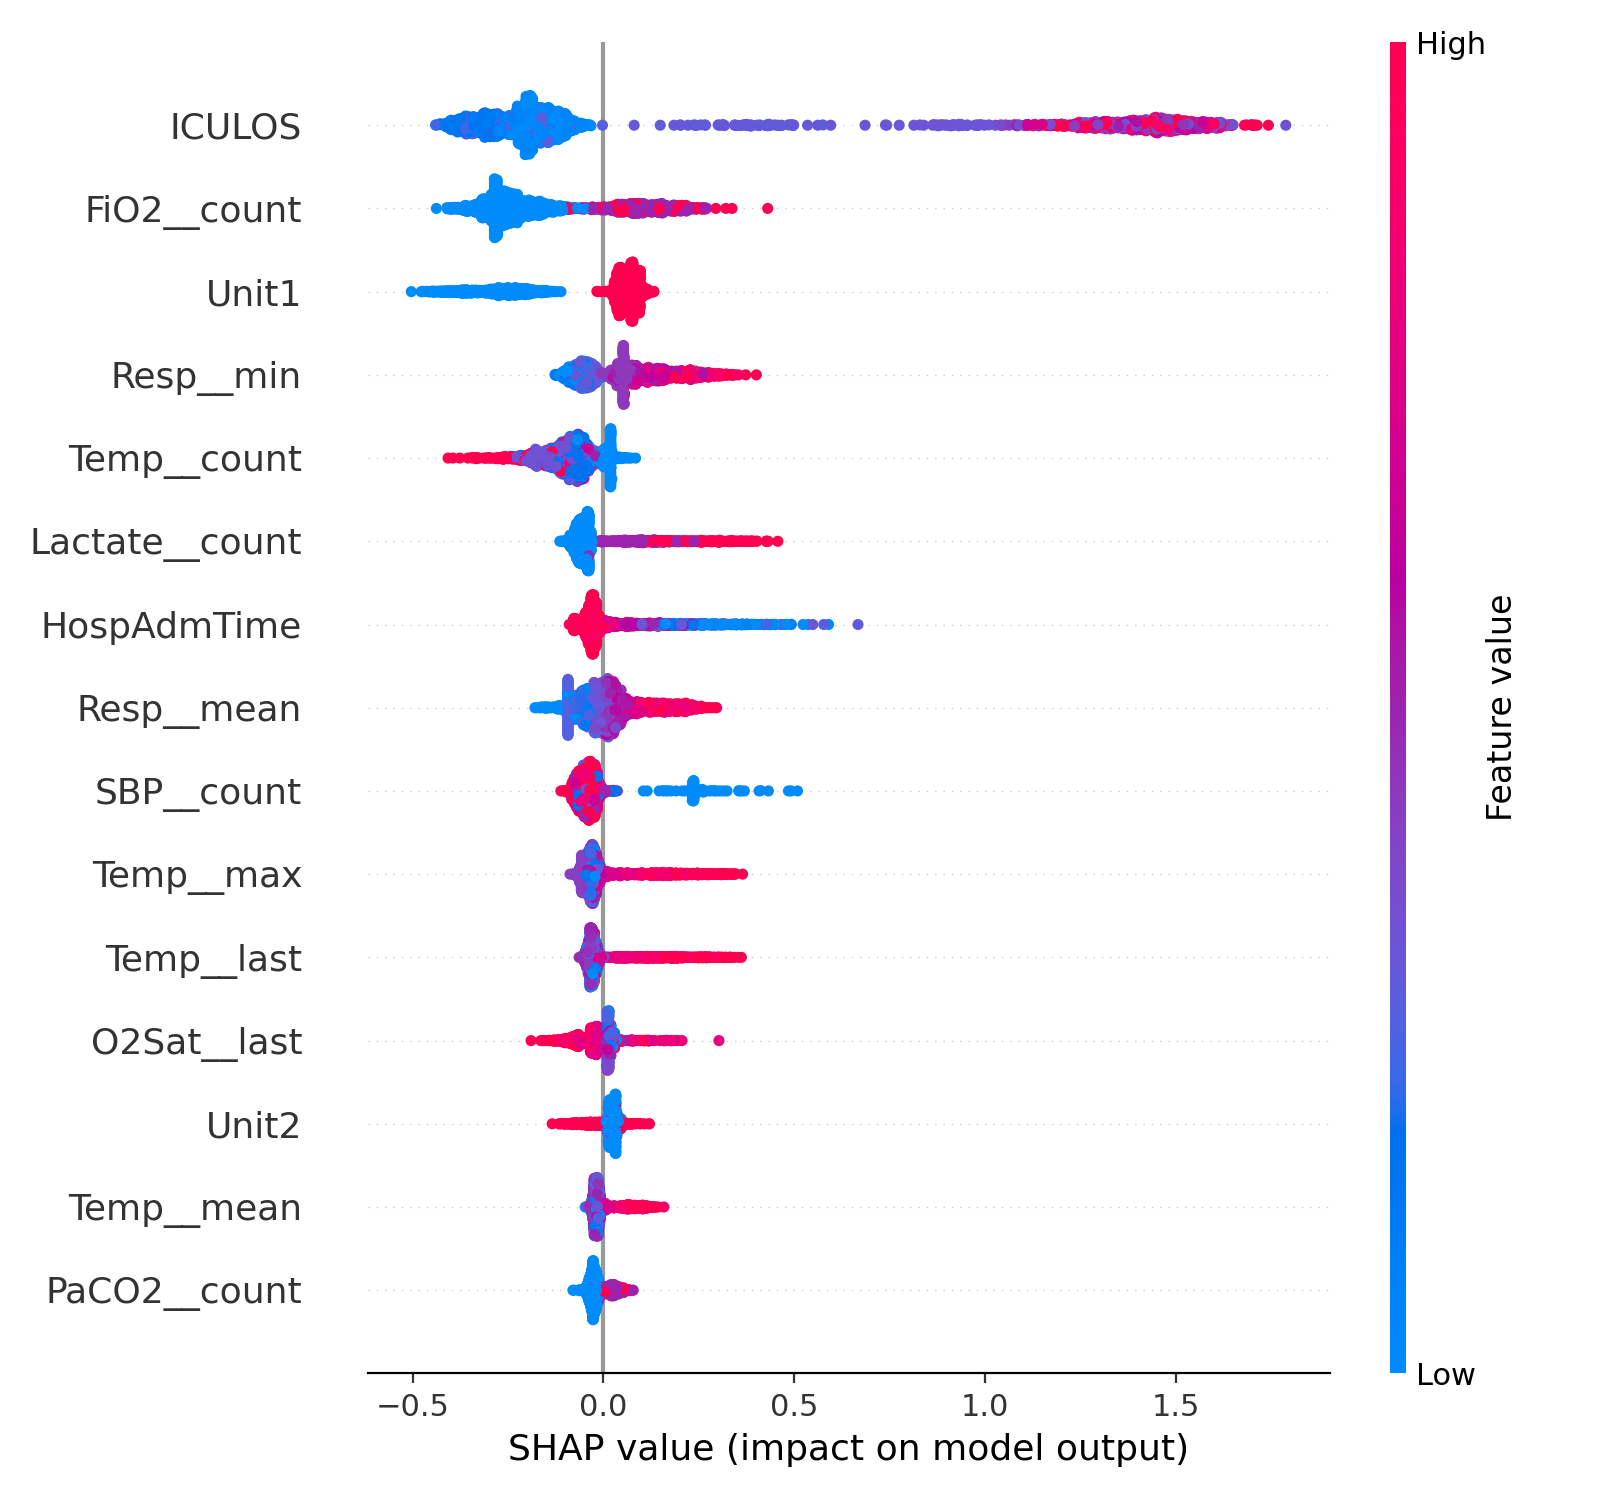
\includegraphics[width=0.95\columnwidth]{figures/shap_summary.png}
\caption{TreeSHAP summary for 2{,}000 test alerts (top 15 features). Each
dot is one alert; colour encodes the feature value and the horizontal
position its contribution to the predicted log-odds of sepsis.}
\label{fig:shap}
\end{figure}

\subsection{Retrieval Quality}
Table~\ref{tab:retr} shows retrieval results for ablations A1 and A2. % State
% whether SHAP-guided queries beat generic and LLM-written queries, by how
% much, and whether the difference is significant.

\begin{table}[!t]
\caption{Retrieval Quality by Query Source and Retriever}
\label{tab:retr}
\centering
\footnotesize
\begin{tabular}{@{}llcc@{}}
\toprule
Query source & Retriever & nDCG@5 & P@5 \\
\midrule
Generic & Hybrid & \tbd & \tbd \\
All abnormal (no SHAP) & Hybrid & \tbd & \tbd \\
LLM-written & Hybrid & \tbd & \tbd \\
\midrule
SHAP-guided & BM25 & \tbd & \tbd \\
SHAP-guided & Dense (BGE) & \tbd & \tbd \\
\textbf{SHAP-guided} & \textbf{Hybrid} & \tbd & \tbd \\
\bottomrule
\end{tabular}
\end{table}

\subsection{Generation Quality and Routing}
Table~\ref{tab:gen} compares correction strategies and graders (A3, A4).
After threshold calibration, the selected values were $\tau_h=\tbd$ and
$\tau_l=\tbd$, and \tbd\%, \tbd\%, and \tbd\% of cases were routed to
\textsc{Correct}, \textsc{Ambiguous}, and \textsc{Incorrect},
respectively. % Interpret: did CRAG raise faithfulness and citation
% precision, and what did it cost in latency?

\begin{table}[!t]
\caption{Generation Quality by Correction Strategy and Grader}
\label{tab:gen}
\centering
\footnotesize
\setlength{\tabcolsep}{3pt}
\begin{tabular}{@{}lcccc@{}}
\toprule
Configuration & Faithf. & Ans. rel. & Cit. prec. & Latency (s) \\
\midrule
Standard RAG & \tbd & \tbd & \tbd & \tbd \\
Grader filter only & \tbd & \tbd & \tbd & \tbd \\
CRAG, MS MARCO grader & \tbd & \tbd & \tbd & \tbd \\
CRAG, MedCPT grader & \tbd & \tbd & \tbd & \tbd \\
\textbf{CRAG, BioBERT grader} & \tbd & \tbd & \tbd & \tbd \\
\bottomrule
\end{tabular}
\end{table}

% ---------------------------------------------------------------------
\section{Discussion}

\subsection{Why Separate the Tasks}
The design rests on matching each sub-problem to a suitable tool. Numeric
risk estimation over dozens of correlated, partially missing variables is a
well-studied tabular problem for which boosted trees are strong,
well-calibrated after post-processing, and exactly explainable through
TreeSHAP. Asking an LLM to perform this step would expose the most
safety-critical output to arithmetic and threshold errors. Conversely, the
LLM is valuable precisely where tabular models are silent: turning graded
evidence into readable text. Restricting the LLM to that role, and checking
its citations afterwards, narrows the space in which unsupported content
can appear.

\subsection{Role of the SHAP-to-RAG Bridge}
Generic queries tend to retrieve broad overview passages on sepsis that are
correct but not specific to the patient in front of the clinician. Using
SHAP drivers ties retrieval to the physiological reasons for the alert, so
two high-risk patients with different drivers---one hypotensive with raised
lactate, another hypoxaemic with leukocytosis---receive different evidence.
The trigger check matters as well: SHAP describes what moved the model, not
what is clinically abnormal, and filtering through the lexicon prevents
queries about normal values that happened to shift the prediction.
% Support or revise this paragraph with your Table VI results.

\subsection{Effect of Corrective Routing}
The three-way routing addresses two different failure modes. When local
coverage is good but passages contain mixed content, strip-level filtering
removes off-topic sentences. When coverage is poor, PubMed fallback
replaces evidence rather than forcing the generator to work with irrelevant
text. The explicit ``insufficient evidence'' outcome is an important safety
property: the system prefers silence to speculation.
% Support or revise this paragraph with your Table VII results.

\subsection{Privacy and Safety Considerations}
Only derived, binned feature descriptions and public evidence are sent to
the generator, and MIMIC-IV experiments run fully offline, consistent with
its data use agreement. The system displays probabilities, drivers, and
sources side by side so that clinicians can verify each claim. It does not
recommend specific drugs or doses, and it is not a certified medical
device.

\subsection{Limitations}
Five limitations bound this study. (1) Labels follow the Sepsis-3-based
definition of a single public benchmark, and performance may differ under
other definitions or populations; the model also relies partly on
non-physiological signals such as ICU length of stay and test-ordering
frequency, which may not transfer across sites. (2) Retrieval relevance is judged by a
small annotator team, so absolute scores carry uncertainty even with
adjudication. (3) RAGAS uses an LLM as judge and does not replace expert
clinical review. (4) The concept lexicon covers common sepsis-related
abnormalities and would need extension for other conditions. (5) Routing
thresholds calibrated on one corpus may not transfer to a different
knowledge base without recalibration.

% ---------------------------------------------------------------------
\section{Conclusion and Future Work}

This paper presented a clinical decision-support pipeline that joins
tabular risk prediction, patient-level explanation, and self-correcting
evidence retrieval. TreeSHAP attributions are not only displayed but are
converted into deterministic, terminology-controlled queries; retrieved
evidence is graded by a biomedical cross-encoder and repaired through
MeSH-based PubMed fallback; and the LLM is limited to citing graded
evidence. On the PhysioNet 2019 cohort with cross-hospital testing, the
selected model achieved an AUROC of 0.800, SHAP-guided queries improved
nDCG@5 by \tbd{}, and corrective routing raised faithfulness by \tbd{}
over standard RAG.

Future work will (1) replace window statistics with sequence models that
capture longer trends; (2) extend the lexicon and evidence corpus to other
deterioration syndromes such as acute respiratory failure; (3) carry out a
structured usability and safety study with practising intensivists; and
(4) integrate with EHR systems through HL7 FHIR for prospective, silent-mode
evaluation.

\subsection*{Reproducibility}
All preprocessing steps are fitted on training data only, splits are made
at patient and hospital level, hyperparameters are fixed before the test
set is used, and random seeds are set to 42. Code is available from the
authors on request.

\section*{Acknowledgement}
The authors thank the Department of Computing Technologies, SRM Institute
of Science and Technology, for infrastructure support, and the maintainers
of PhysioNet for providing open access to the challenge data. We also
acknowledge the open-source communities behind scikit-learn, LightGBM,
SHAP, ChromaDB, and LangGraph.

\bibliographystyle{IEEEtran}
\bibliography{references}

\end{document}
